\documentclass[main.tex]{subfiles}
\begin{document}

\chapter{General introduction}
\thispagestyle{chapstyle}
\minitoc



\section{Context}
This document presents the work I carried-out during my CIFRE PhD with Airbus and ONERA. The main purpose of this study is to assess the suitability of many-core processors to meet the needs and constraints of future avionics systems.
Overall, the context of this thesis is threefold. Firstly, the \emph{avionics} context imposes safety-requirements regarding the design of systems, including software development tasks and certification-related issues. Secondly, the \emph{industrial} context brings needs for high computational power on-board in order to design more performant and more cost-efficient aircrafts. And finally, the \emph{technological} context offers new perspectives for the design of future embedded systems thanks to promising emerging technologies.


\subsection{Avionics context}
Aircrafts must be safe and this entails that all systems having a potential impact on the flight safety are required to meet stringent safety-related constraints. When it comes to developing safety-critical software, several safety-related constraints need to be met during design, implementation, verification and test phases of the software's life cycle.


\subsubsection{Safety requirements on software}
Software issues unfortunately happened to be the root cause of several system failures causing the loss of human lives in the past. For example, in 1992, the anti-missile {\sc Patriot} failed to intercept an incoming missile because of accumulated errors in floating point calculations~\cite{MissilePatriot}. As a result, 28 soldiers were killed and approximately 100 persons were injured. More recently, an Airbus A400M crashed during takeoff, killing all the crew on board~\cite{CrashA400M}. Investigations revealed that an incorrect installation of the engine control software during production may have caused three out of four engines to stop responding to throttle commands, thus causing the accident.

In order to increase the confidence in all safety-critical systems used in aircrafts, constraints have been imposed to aircraft manufacturers. In particular, all safety-critical systems are legally required to be \emph{certified} by independent authorities to be granted operational flight permission.

\subsubsection{Software certification}
Civil aviation is ruled by independent legal authorities. Before operational use, aircrafts are examined by the authorities to verify their safety. More precisely, manufacturers are expected to demonstrate the compliance of the aircraft with the authority's regulations to obtain \emph{certification} and be permitted to fly civilians. Today, these regulations are mainly communicated with specific industry standards including the ARP-4754~\cite{arp4754} regarding system development, the DO-254~\cite{do178} regarding hardware development life cycle and the DO-178C~\cite{do178} for the software development life cycle.
Overall, the requirements imposed on designs depend on the \emph{Design Assurance Level} (or \emph{DAL}) of the system under consideration. Table~\ref{tab_intro_DALs} is extracted from the ARP-4761~\cite{arp4761} and provides a description of the five DALs. Naturally, developing high assurance software requires higher efforts since design, implementation, verification and testing are constrained in the DO-178C. 
Overall, software certification is mostly process-driven. As the rationale, it can be argued that properly developed software has higher chances of being correct. Yet, some of the constraints of the DO-178C do not only change the development process but also change the actual design choices of the system overall. For example, DO-178C requires that applicants compute the Worst Case Execution Time (or WCET) of software programs. Computing non pessimistic WCETs is a difficult task on modern processors. Being able to compute them efficiently on even more complex processors in the future is a challenge that needs to be tackled.



\begin{table}
    \centering  
    {
    \small
    \begin{tabularx}{\textwidth}{cccX}
	\hline
        {\sc \textbf{Level}} 	& {\sc \textbf{Proba.}} & {\sc \textbf{Severity}} & {\sc \textbf{Failure condition effect}}	\\
	    \hline
        DAL - A & $10^{-9}/h$ & Catastrophic & All failure conditions which prevent continued safe flight and landing \\
        
        \hline
        DAL - B & $10^{-7}/h$ & Hazardous    & Large reduction in safety margins or functional capabilities; higher workload or physical distress such that the crew could not be relied upon to perform tasks accurately or completely; adverse effects upon occupants\\

        \hline
        DAL - C & $10^{-5}/h$ & Major        & Significant reduction in safety margin or functional capabilities; significant increase in crew workload or in conditions impairing crew efficiency; some discomfort to occupants\\

        \hline
        DAL - D & $10^{-3}/h$ & Minor        & Slight reduction in safety margin; slight increase in crew workload; some inconvenience to occupants \\

        \hline
        DAL - E &   N/A       & No effect    & None \\
        \hline	
\end{tabularx}
    }
    \caption{Description of the Design Assurance Levels from the ARP-4761~\cite{arp4761}}
    \label{tab_intro_DALs}
\end{table}


Overall, the avionics context enforces safety-related constraints on the design of software. In particular, certification problems lead to complex development processes and stringent constraints on demonstrability. Proving adherence to the standards will remain a necessity for future designs. Thus, deep software changes will be possible only if demonstrability and development processes can comply with the requirements of authorities.


\subsection{Industrial context}
When aircrafts are designed, safety is incontestably the highest priority. Yet, in an industrial context, manufacturers try to optimize performance and cost as much as possible without compromising safety. We detail the consequences on the design of embedded avionics computers below.

\subsubsection{Needs in computational power}
The need in embedded computational power within aircrafts is growing slower than in other areas of computer science. Yet, it still grows exponentially. Historically, new embedded computers were introduced to execute the flight control systems of each of the following aircrafts: A320 (first flight in 1987), A340 (first flight in 1991), A340 with new engines (first flight in 2001), A380 (first flight in 2005) and A350 (first flight in 2013). For each new generation, the need in computational power has been multiplied by a factor comprised between 2 and 3 in comparison with the previous generation. When looked over the past 25 years, this factor becomes close to 50. Such a raise is essentially motivated by evolutions in the control laws to either increase flight safety or reduce the aircraft's weight. For example, the \emph{Gust Load Alleviation} (or \emph{GLA}) method implemented in the A350 enabled to reduce the metal fatigue of the mechanical structure and thus to decrease its weight by 400 kilograms. In this case, the introduction of GLA required to add new elements to the control laws, to significantly increase the frequency at which incidence is measured, to meet short latency requirements at run-time and to implement thorough monitoring of the new parts of the system. Clearly, if GLA helped improve the A350's performance, it also came at the cost of an extra load on the CPU. Other evolutions of the flight control system alleviated the efforts on the mechanical structure such as the reduction of the rudder's oscillation tolerance on the A350. Again this enabled a significant reduction of the aircraft's weight and improved its performance overall. However, it also increased the computational work-load because of the additional complexity in the control laws, because of the new monitoring features that were required and because of the new entries introduced at system level.
While it is clear that flight control systems are becoming more and more demanding, the growing need in computational power is shared more globally by many different systems in the aircraft. Currently, the cockpit-related systems are driving several innovation efforts which all rely on more electronics and more software components. Engineers investigate the feasibility of new features to improve many aspects of the aircraft, including maintenance problems or flying aids for pilots.
And finally, promising technologies leveraging machine learning algorithms are now available to solve linear and logistic regression problems, to compress data using dimensionality-reduction, or to apply clustering techniques on large sets of data in a wide range of industries. While not currently in use, such algorithms are likely to find their path to aerospace applications in the future. One of the key challenge here will be to bring sufficient computational resources on-board to process these potentially massive, but often parallel, work-loads.

Overall, the needs for more powerful computers in aircrafts is growing from all sides. At the same time, industrial trends converge towards more integrated architectures where the same execution target can host the software parts of several systems. This concept of resource sharing is most commonly known as the concept of \emph{Integrated Modular Avionics}.




\subsubsection{Integrated Modular Avionics}
Aircrafts embed many different systems. From the A300 and until the A340-500, Airbus' aircrafts used to feature one specific \emph{Line Replaceable Unit} (or \emph{LRU}) to support each and every function. A LRU is a dedicated embedded computer which is manufactured by a system supplier in order to process the software components of a system. With the exponential growth of functionality demands from airlines, aircrafts manufacturers concluded during the nineties that such an approach where the number of embedded computers grows exponentially could not be reasonably sustained any more. To tackle this issue, the concept of Integrated Modular Avionics (or IMA) was introduced. Honeywell firstly used it in 1995  for the cockpit functions of the Boeing 777 aircraft\footnote{This was the first IMA in a \emph{civil} aircraft - IMA were already in use in several jet fighters such as the F-22, the F-35 or the Dassault Rafale at that time.}. Few years later, Airbus and Thales extended the concept during the design of the A380 with the introduction of the \emph{Open IMA}. Today, the concept of IMA is becoming a standard that is used in most modern civil aircrafts such as the Boeing 787 Dreamliner and the Airbus A350. 

\begin{figure}
    \centering

    \begin{subfigure}[b]{0.49\linewidth}
        \scalebox{0.9}{
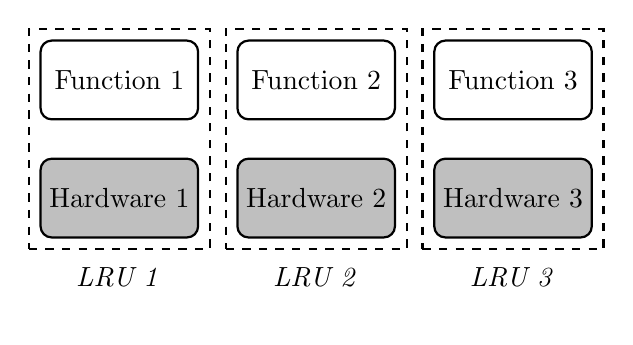
\begin{tikzpicture}[font={\fontsize{10pt}{12}\selectfont}]

    \node[rectangle, draw, color=black, thick, anchor=south west, minimum width=2.3cm, minimum height=2.8cm, inner sep=0pt, dashed]  at (-0.15, -0.15) {};
    \node[anchor=south west, minimum width=2cm, minimum height=1cm, inner sep=0pt]  at (0, -1) {\emph{LRU 1}};

    
    \node[rectangle, draw, color=black, thick, anchor=south west, minimum width=2.3cm, minimum height=2.8cm, inner sep=0pt, dashed]  at (2.35, -0.15) {};
\node[anchor=south west, minimum width=2cm, minimum height=1cm, inner sep=0pt]  at (2.5, -1) {\emph{LRU 2}};
    

    \node[rectangle, draw, color=black, thick, anchor=south west, minimum width=2.3cm, minimum height=2.8cm, inner sep=0pt, dashed]  at (4.85, -0.15) {};
\node[anchor=south west, minimum width=2cm, minimum height=1cm, inner sep=0pt]  at (5, -1) {\emph{LRU 3}};
    

    \node[rectangle, draw, color=black, rounded corners, thick, anchor=south west, minimum width=2cm, minimum height=1cm, inner sep=0pt, fill=lightgray]  at (0, 0) {Hardware 1};
    \node[rectangle, draw, color=black, rounded corners, thick, anchor=south west, minimum width=2cm, minimum height=1cm, inner sep=0pt, fill=lightgray]  at (2.5, 0) {Hardware 2};
    \node[rectangle, draw, color=black, rounded corners, thick, anchor=south west, minimum width=2cm, minimum height=1cm, inner sep=0pt, fill=lightgray]  at (5, 0) {Hardware 3};

    \node[rectangle, draw, color=black, rounded corners, thick, anchor=south west, minimum width=2cm, minimum height=1cm, inner sep=0pt]  at (0, 1.5) {Function 1};
    \node[rectangle, draw, color=black, rounded corners, thick, anchor=south west, minimum width=2cm, minimum height=1cm, inner sep=0pt]  at (2.5, 1.5) {Function 2};
    \node[rectangle, draw, color=black, rounded corners, thick, anchor=south west, minimum width=2cm, minimum height=1cm, inner sep=0pt]  at (5, 1.5) {Function 3};
\end{tikzpicture}
}
        \caption{Federated approach}
        \label{fig_intro_federatedApproach}
    \end{subfigure}
    \begin{subfigure}[b]{0.49\linewidth}
        \centering
        \scalebox{0.9}{
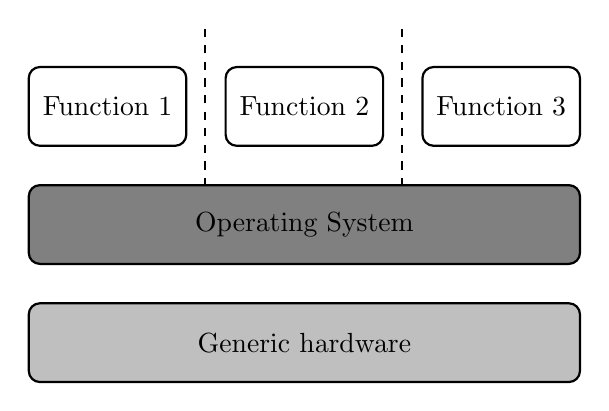
\begin{tikzpicture}[font={\fontsize{10pt}{12}\selectfont}]
    
    \node[rectangle, draw, color=black, rounded corners, thick, anchor=south west, minimum width=2cm, minimum height=1cm, inner sep=0pt]  at (0, 1.5) {Function 1};
    \node[rectangle, draw, color=black, rounded corners, thick, anchor=south west, minimum width=2cm, minimum height=1cm, inner sep=0pt]  at (2.5, 1.5) {Function 2};
    \node[rectangle, draw, color=black, rounded corners, thick, anchor=south west, minimum width=2cm, minimum height=1cm, inner sep=0pt]  at (5, 1.5) {Function 3};
    

    \node[rectangle, draw, color=black, rounded corners, thick, anchor=south west, minimum width=7cm, minimum height=1cm, inner sep=0pt, fill=gray]  at (0, 0) {Operating System};
    
    \node[rectangle, draw, color=black, rounded corners, thick, anchor=south west, minimum width=7cm, minimum height=1cm, inner sep=0pt, fill=lightgray]  at (0, -1.5) {Generic hardware};

    \draw[thick, dashed] (2.25, 1) -- (2.25, 3);
    \draw[thick, dashed] (4.75, 1) -- (4.75, 3);
    
\end{tikzpicture}
}
        \caption{Integrated Modular Avionics}
        \label{fig_intro_IMA}
    \end{subfigure}
    \caption{Comparison of federated and IMA architectures}
    \label{fig_intro_comparisonFederatedVsIMA}
\end{figure}

As shown in Figure~\ref{fig_intro_comparisonFederatedVsIMA}, the idea of IMA is to enable several applications to be hosted on a single generic platform. By sharing hardware resources (usually with COTS processors), the number of embedded computers can be decreased and so do their weight, their production and design costs and their maintenance efforts. Yet sharing those resources also brings interesting technical challenges to ensure robust partitioning between systems. Indeed, functions often need to be independent from each other and co-hosting their software parts requires to meet stringent temporal-isolation constraints. Systems with different criticality levels can be safely co-hosted on a single target if and only if failures of low-criticality systems cannot propagate to those with higher DAL. And finally, it is required for cost reasons that, despite a shared hardware, software systems can be developed, tested and \emph{certified} independently from each other. The possibility of certifying software components independently enables \emph{incremental certification} and greatly narrows certification costs.
%ARINC-653~\cite{arinc653}

Overall, the industrial context of this thesis brings two different challenges regarding the design of future avionics computers. The growing demand of computational power from applications needs to be met while, in the context of IMA systems, the property of robust partitioning between applications also needs to be ensured. Clearly, tackling these two issues simultaneously will become increasingly hard as applications grow and as execution targets are more and more shared. The emergence of new processors appears as a great opportunity to respond to the need for such computationally-efficient and computationally-shareable processors.




\subsection{Technological context}
Nowadays, the architectural paradigm upon which modern micro-processors are designed is evolving. The transistor density gains from Moore's Law~\cite{Moore1975} and the transistor speed growth both face technological limits bringing new challenges for the strive for computational performance. Deep changes in processor architectures already occurred in the past. Multi-core processors were introduced to beat the inflexion of performance scaling when pure architectural optimizations with pipelining, speculative branching or out-of-order execution were seen as the main solutions to increase performance.
Today, traditional multi-core architectures are again facing difficulties to keep scaling up computational power at a reasonable energetic cost. As technological limits regarding transistor size and frequencies are close to be reached, designs are forced to rely on new architectures to sustain the pace at which performance needs are growing. In this context, new processors architectures featuring massively parallel processing arrays are now emerging. These processors are usually referred to as \emph{many-core} processors.

\subsubsection{Towards many-core processors}
Recently, the design of \emph{parallel} processors gained a lot of attention. As shown in Figure~\ref{fig_intro_procPerfScaling}, the number of transistors in micro-processors has sustained Moore's Law over the past 25 years. However, it is clear that the raw sequential computational power of cores changed with the introduction of multi-core processors around 2004. The motivation for this change is related to the energetic profitability of adding further complex sequential optimization mechanisms to already complex pipelined, cached and speculative core architectures~\cite{Borkar2011}. In multi-core processors, several computing cores and their peripherals (ex: DDR-SDRAM controllers, Ethernet controllers, ...) are typically interconnected by either a shared bus or a crossbar. Although such architectures successfully increased the computational power of micro-processors, it appears that, in both cases, scaling up the number of cores to hundreds or thousands now raises important issues. In cases of buses, concerns are related to performance balance of the cores vs the bus. In the case of crossbars, concerns are related to their exponential cost as the number of end-points grows.

\begin{figure}
    \centering
    \includegraphics[width=14cm]{imgs/png/intro_procPerfScaling.png}
    \caption{Logarithmic comparison of transistor count, frequency, power, performance and number of cores in micro-processors between 1985 and 2010 (extracted from~\cite{Fuller2011})}
    \label{fig_intro_procPerfScaling}
\end{figure}

To overcome this issue, the concept of \emph{tiled} architectures has been introduced~\cite{Taylor2007}. Tiled microprocessors rely on several independent computing tiles interconnected by a Network-on-Chip (or NoC) rather than a bus or a crossbar. By doing so, the architecture becomes scalable and allows to design processors with hundreds or even thousands of cores on a single chip. Those processors are referred to as the many-core processors. While they have been available only in research environments for few years, some of them are now available on the market.



\subsubsection{COTS many-core processors}
The market of \emph{Commercial off-the-shelf} (or \emph{COTS}) many-core processors is growing. Today, two main categories of many-core processors are available. Firstly, those dedicated to unload a main processor from some of its tasks and to run as a side processor. The Intel Xeon Phi~\cite{XeonPhi} family is a typical example of this category. Xeon Phi co-processors are available upon a variety of configurations with up to 72 cores consuming more than 200W. This order of magnitude in energy consumption is usually not suitable for embedded systems. 

The Adapteva Epiphany~\cite{Epiphany} co-processor also falls in the same category, but with a better energetic consumption. Unfortunately, it does not feature enough computational power for the kind of applications targeted in thesis under it 16 cores configuration. 

This category may also include the \emph{Graphical Processing Units} (or \emph{GPUs}), especially if they can be used to process general purpose programs using OpenCL~\cite{OpenCL} or CUDA~\cite{CUDA} for example. Yet, GPU are usually designed following the \emph{Single Instruction Multiple Data} (or \emph{SIMD}) philosophy which is not well suited to process several independent programs. We argue that \emph{Multiple Instruction Multiple Data} (or \emph{MIMD}) processors are better suited to our needs. \\


The second category of many-core processors is composed of those which can be used as main processors in a computer. Historically, the Intel Single-chip Cloud Computer (or \emph{SCC})~\cite{intel_scc} was probably one of the first many-core processor of that type available. With 48 cores and a potentially low (depending on frequency scaling) power consumption, the SCC is an interesting platform for our needs. Unfortunately, it has been designed only for research purposes and will not be used in any industrial product.

In the same category, the Tile Gx*~\cite{TileGx} and Mx*~\cite{TileMx} families from Mellanox (formerly Tilera, then EZchip) feature up to 72 and 100 processing cores respectively. This provides them with massive computational power. Unfortunately, although fairly low already, their thermal dissipation power is still too high to design electronics boards with only passive cooling. Even if it is not an absolute necessity, avoiding active cooling is an asset to design boards which do not require additional certification of the cooling system.

In contrary, the \mppalong~\cite{kalray_mppa} processor offers a good energetic consumptions which, under specific configurations, may be sufficiently low to avoid the problem of active cooling. With 288 cores, its raw computational power is also massive. Clearly, the \mppalong is an interesting candidate given our needs and constraints.


\section{Thesis motivations}
In an avionics context where software must be safe and certified, and an industrial context where heavy workloads need to be hosted on shared platforms, massively parallel processors such as the \mppalong offer interesting opportunities for the design of future avionics computers. Their raw computational power may theoretically enable to speedup on-board processing by a high factor, thus leaving either time for other applications to run or large margins on the timing constraints of applications. However, getting there involves to tackle several technical challenges first.


Firstly, bounds on the execution times of safety-critical software components must be found to meet certification criteria. Unfortunately, computing WCETs is getting harder as hardware complexity increases. In particular, it is well known from previous works on multi-core processors that, with parallel software, the main problems for computing WCETs lie in the management of shared resources. On massively parallel processors, some resources are massively shared. Consequently, mitigating the impact of shared resources on the execution time bounds will be a first challenge to overcome.

Secondly, the distributed architecture of many-core processors increases their programming complexity. The \mppalong has a hierarchical architecture with several types of peripherals, memories, NoCs and cores. In a safety-critical context where software designers must have total control of the hardware, being able to program and to configure all parts of the processor at a very low level is especially challenging.


Finally, the cost of handmade mapping of applications on a many-core processor can quickly become prohibitive, especially when the targeted applications are large and complex. Tools automatically achieving this work would be a considerable asset to make many-core processors usable in an industrial context. However, the design of such tools is challenging since not only all the caveats of the target must be taken into account, but also because the approach is required to scale up to industrial-sized problems and to provide results in reasonable amounts of time.\\

%Tackling these technical issues justifies this thesis.

\section{Approach}
As explained below, we propose to address the challenges listed above with an approach relying on three pillars. Firstly, regarding the problem of shared resources, we propose a thorough analysis of the architectural details of the \mppalong. Based on this analysis, we provide an \emph{execution model} limiting access to shared resources by applications to strict pre-defined boundaries. In particular, we focus on the management of three types of hardware resources that have a major impact on performance and predictability, namely the local memories, the NoC and the external DDR-SDRAM. Controlling the behaviour of applications when accessing those resources enables to isolate applications from each other, and thus to compute their WCETs without excessive pessimism. Moreover, being able to isolate applications is a very desirable property in the context of IMA systems.

Secondly, regarding the problem of programming complexity, we propose a \emph{hypervisor} that implements the principles stated by our execution model. This hypervisor is developed in bare-metal on the \mppalong, and manages all resources under consideration. In particular, it manages the NoC and it enables the execution of applications that are distributed over several NoC end-points. Moreover, it enforces the respect of the execution model's rule at run-time and prevents propagation of faults between isolated applications. The validation of hypervisor is achieved using experimental benchmarks. Overall, this development work not only demonstrates that using many-core processors can be made easier with an appropriate hypervisor, it also forms an execution framework enabling distributed applications to run, and thus to exploit all the computational power of a massively parallel architecture.

Finally, we fix the issue of mapping large applications on the \mppalong automatically using constraint programming. We provide formal models of applications, of the hardware platform and of the needs for resources from applications. Based on this, we formulate the mapping problem using a modern solver and we perform extensive parametric studies to evaluate the capability of our approach to deal with a large industrial application provided with many different sets of resources. Overall, we show that, using constraint programming efficiently, mapping large and constrained applications on many-core processors can be done automatically and formally in a reasonable amount of time.


\section{Content of the dissertation}
The remainder of this dissertation is structured as follows. 
Chapter~\ref{chap_systemModel} clarifies the inputs of this thesis. This includes the model of applications and details about the COTS many-core processor under consideration. Moreover, constraints inherited from the industrial context are described in further details.
Chapter~\ref{chap_boundingExecTimes} and Chapter~\ref{chap_schedParallelTasks} review the state of art regarding predictable execution on multi- and many-core processors. The former covers the techniques employed to bound the execution times of programs while the latter focuses on scheduling and mapping problems on parallel architectures.
Chapter~\ref{chap_execModel} details and motivates the use of an execution model to master the access to shared resources and thus to improve predictability. Chapter~\ref{chap_framework} describes how the property of temporal isolation provided by the execution model can be leveraged to design a many-core integration work-flow. Overall it enables multiple parallel applications to be designed, implemented, verified and tested independently despite sharing hardware resources. 
Chapter~\ref{chap_implemExecMod} details how the applications are isolated on-line using a hypervisor that implements the rules of the execution model. Chapter~\ref{chap_budgetValidation} provides a solution to the problem of automatically mapping applications on some of the resources of many-core processor.
Finally, Chapter~\ref{chap_conclu} summarises the contributions of this thesis and outlines possibilities of future work.





\clearpage
\subbiblio
\end{document}
